\chapter{系统实现与实验评价}\label{chap:evaluation}

本章主要阐述基于 FPGA 的 SLAM 后端加速系统的实验平台与环境搭建，并通过一系列定量实验验证系统的有效性。实验评估围绕轨迹精度、计算延迟与加速比、资源利用率、功耗与能效以及 SOB 编码优化效果展开，并在公开数据集与真实场景下进行综合验证。

\section{实验平台与环境搭建}

本节详细介绍实验所采用的硬件平台配置、软件系统架构设计以及用于验证的数据集基准。为了验证软硬协同加速方案的有效性，实验构建了一套涵盖底层 FPGA 逻辑、嵌入式运行时环境与上层应用框架的完整测试系统。

\subsection{硬件平台配置}

本文实验平台采用赛灵思（Xilinx）Zynq UltraScale+ MPSoC 系列开发板，覆盖实验评估与真实场景验证两类硬件环境。整体硬件系统的 Block Design 遵循高吞吐量、低延迟的设计原则，通过 AXI 高性能总线实现 PS 端与 PL 端的紧耦合互联。

\subsubsection{评估平台 (ZCU106)}

离线性能评估与资源统计在 ZCU106 开发板上完成（如图~\ref{fig:hetero_platform} 所示）。该平台集成四核 ARM Cortex-A53 处理器与大规模可编程逻辑资源，能够稳定支撑后端加速器的软硬协同验证。ZCU106 平台的主要硬件配置如下：
\begin{figure}[h!t]
\centering
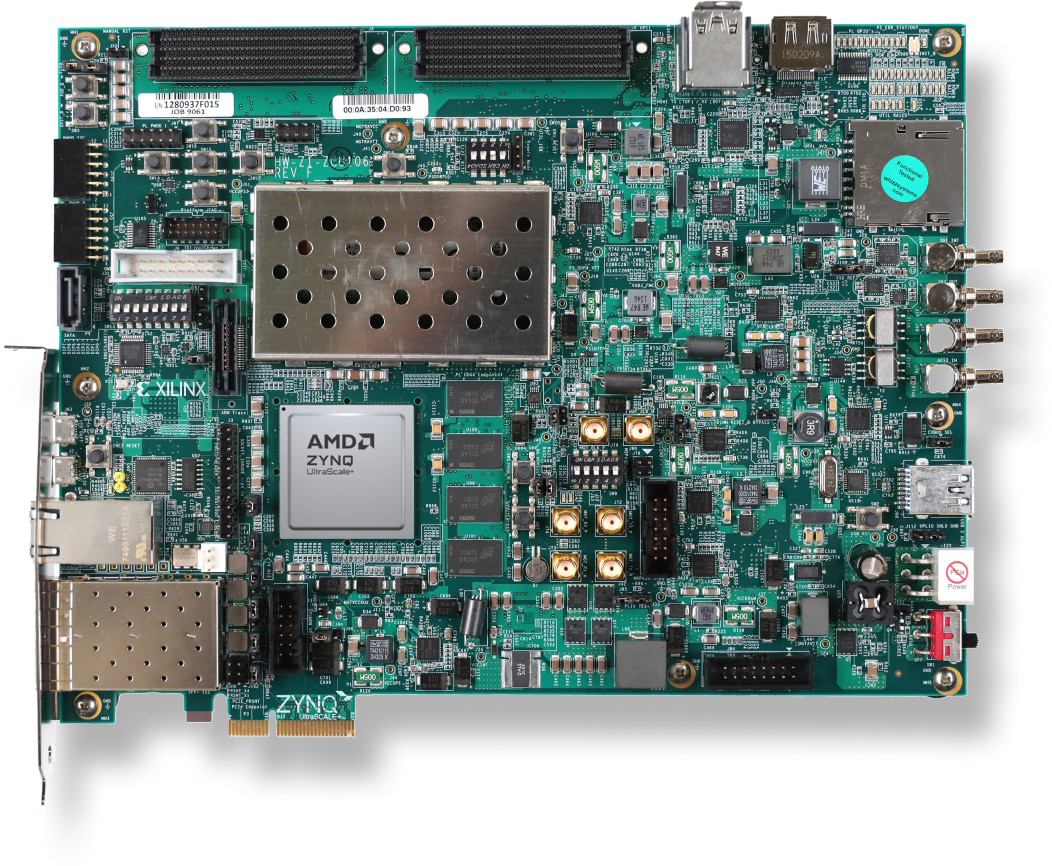
\includegraphics[width=0.9\linewidth]{Img/zcu-106.jpg}
\bicaption{评估平台 ZCU106 实物图}{Physical view of the ZCU106 evaluation platform}
\label{fig:hetero_platform}
\end{figure}
\begin{itemize}
    \item 处理器系统（PS）：四核 ARM Cortex-A53，最高频率 1.2~GHz，配备 4~GB DDR4 内存。
    \item 可编程逻辑（PL）：约 1143K 逻辑单元（Logic Cells）与 2520 个 DSP 计算切片。
\end{itemize}

\subsubsection{应用平台 (XCZU19EG)}

真实场景测试部分使用集成式异构计算板卡（如图~\ref{fig:application_platform} 所示），其核心器件为 XCZU19EG。该平台在 PS 端同样采用 Cortex-A53 架构，PL 端提供更充足的逻辑单元与片上存储资源。为了满足真实场景下高动态定位的需求，板卡集成了高性能的视觉与惯性传感器：

\begin{figure}[h!t]
\centering
\includegraphics[width=0.9\linewidth]{Img/application_platform.png}
\bicaption{异构计算应用平台 (XCZU19EG) 实物图}{Physical view of the XCZU19EG application platform}
\label{fig:application_platform}
\end{figure}

\begin{itemize}
    \item \textbf{视觉传感器}：采用安森美（ON Semiconductor）AR0144AT 图像传感器。该传感器为 1/4 英寸 1.0 MP CMOS，分辨率为 $1280 \times 800$。其核心特性是采用全局快门（Global Shutter）像素设计，专为捕捉高速运动场景优化，能够产生清晰、低噪声的图像，有效避免卷帘快门带来的几何畸变，确保前端特征追踪的精度。双目相机模组的物理基线长度（Baseline）设置为 100~mm，以平衡深度估计的精度与测量范围。
    \item \textbf{惯性测量单元（IMU）}：选用 TDK InvenSense ICM-20948 芯片。这是一款超低功耗的 9 轴运动追踪设备，集成 3 轴陀螺仪、3 轴加速度计和 3 轴磁力计。它内置 16 位 ADC，支持可编程数字滤波器，并通过 7~MHz 高速 SPI 接口与 FPGA 通信，为 VIO 系统提供高频且精确的惯性测量数据。
\end{itemize}

值得注意的是，该平台通过 PL 端逻辑实现了 FSYNC 硬件同步：将按照 IMU 采样时钟生成的 FSYNC 触发信号直接连接至图像传感器的外触发引脚，使图像采集的曝光中心时刻与 IMU 的采样时刻在硬件微秒级层面对齐。该机制极大地减小了视觉与惯性数据之间的时间偏移（Time Offset），为后端基于 Schur Complement 的紧耦合位姿估计提供了高质量、时间同步的观测数据输入。

两类平台均采用统一的软硬划分方式，保证实验结果的可比性。

\subsection{软件系统架构}

为了提高开发效率并实现算法的灵活部署，软件环境基于 PYNQ 3.0.1 框架构建。PYNQ 利用 Python 的生产力优势与 FPGA 的硬件性能，通过 Overlay 机制实现比特流的动态加载与 API 封装。系统的软件栈架构设计如图~\ref{fig:software_arch} 所示，具体包括：

\begin{figure}[h!t]
    \centering
    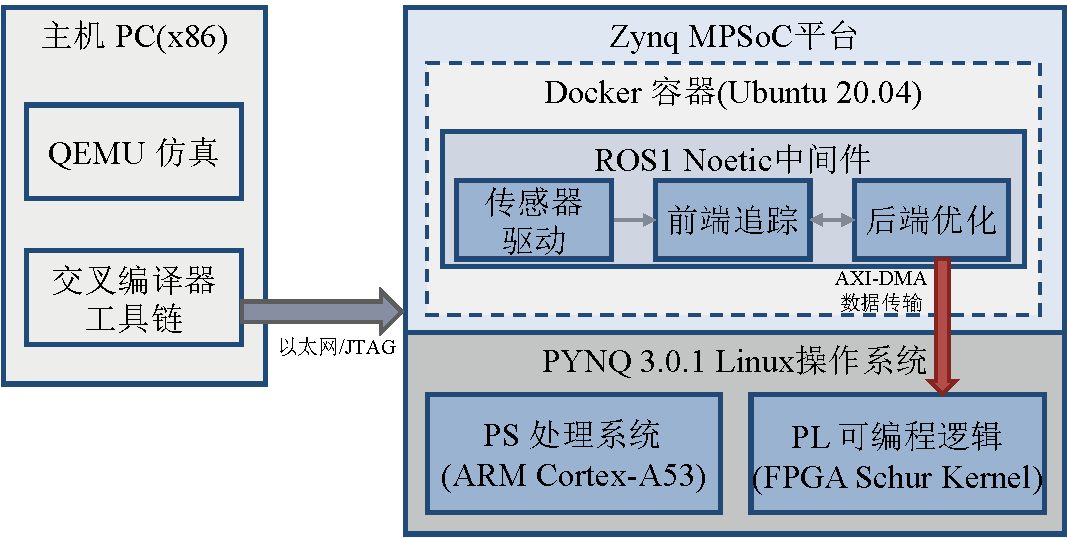
\includegraphics[width=0.95\linewidth]{Img/software_arch_system.png}
    \bicaption{基于 PYNQ 与 Docker 的软件系统架构}{Software system architecture based on PYNQ and Docker}
    \label{fig:software_arch}
\end{figure}

\begin{itemize}
    \item \textbf{操作系统与容器化部署}：宿主机运行基于 PYNQ 3.0.1 的 Linux 系统。为隔离开发环境与依赖库，采用 Docker 技术构建了轻量级且独立的运行环境。容器内部署 Ubuntu 20.04 LTS 镜像，并预装了 ROS、Ceres Solver、Eigen 等 SLAM 核心依赖库。
    \item \textbf{SchurVINS 算法框架集成}：系统选用 SchurVINS 作为 VIO 算法载体。SchurVINS 是一种基于舒尔补的高效视觉惯性里程计框架\cite{fan2024schurvins}，天然契合本文提出的后端加速策略。在移植过程中，我们将原有的 CPU 端舒尔消元线程替换为对 FPGA 加速器的调用接口。
    \item \textbf{ROS 节点管理}：通过 ROS1 Noetic 进行系统层面的节点管理与通信。系统主要包含传感器驱动节点、前端特征追踪节点与后端优化节点。各节点间通过 ROS Topic 传输图像与 IMU 消息，保证了模块间的解耦。
    \item \textbf{交叉编译与仿真}：为了在 x86 主机上加速嵌入式代码的开发，利用 QEMU 模拟器搭建了 ARM64 虚拟环境。该环境允许在 PC 端验证算法逻辑与库兼容性，随后通过交叉编译工具链生成目标平台的可执行文件。
\end{itemize}

\subsection{数据集与测试基准}

软件基准在编译时开启 \texttt{-O3} 级别优化，以确保对比公平性。实验数据采用 EuRoC MAV 数据集与 TUM-VI 数据集，二者均提供精确地面真值轨迹，可用于定量评估系统的定位精度与计算延迟。

EuRoC MAV 数据集由微型飞行器在室内工业环境中采集，提供已同步的双目图像、IMU 测量与高精度轨迹真值\cite{Burri25012016}。数据集包含 11 个工厂场景序列，覆盖从光照良好且运动平缓到运动模糊与弱纹理条件下的快速机动，能够系统性评估视觉惯性系统在复杂动态条件下的精度与鲁棒性。序列命名中的 easy、medium 与 difficult 分别对应不同的飞行难度等级，难度越高意味着更剧烈的运动与更不利的视觉条件。表~\ref{tab:euroc_sequences} 给出了各序列的轨迹长度统计，用于后续误差归一化与性能对比。

\begin{table}[h!t]
\centering
\bicaption{EuRoC MAV 数据集序列与轨迹长度}{EuRoC MAV sequences and trajectory lengths}
\label{tab:euroc_sequences}
\scriptsize
\begin{tabular}{lccccccccccc}
\toprule
序列名称 & MH\_01 & MH\_02 & MH\_03 & MH\_04 & MH\_05 & V1\_01 & V1\_02 & V1\_03 & V2\_01 & V2\_02 & V2\_03 \\
\midrule
轨迹长度（m） & 80.6 & 73.5 & 130.9 & 91.7 & 97.6 & 58.6 & 75.9 & 79.0 & 36.5 & 83.2 & 86.1 \\
\bottomrule
\end{tabular}
\end{table}

TUM-VI 数据集覆盖多种室内场景与运动模式，是面向视觉惯性里程计评测的公开基准\cite{schubert2018vidataset,klenk2021tumvie}。数据集提供 20~Hz 的相机序列与 200~Hz 的 IMU 三轴加速度/角速度测量，传感器在硬件层完成时间同步，并给出经过校准的光度与时间戳信息。为轨迹评估，数据集提供高频率的运动捕捉真值，并将其与相机与 IMU 测量精确对齐，从而支持高精度的轨迹误差分析。本文使用的图像分辨率为 512\,$\times$\,512，以适配嵌入式平台的带宽与计算约束。

TUM-VI 序列包含房间与走廊等典型室内场景，其中房间序列在全程提供真值轨迹，走廊序列在起止段提供真值轨迹，并覆盖不同纹理与视野结构。本文仅选取其中的走廊与室内场景序列用于测试，以覆盖结构化长廊与一般室内空间两类典型环境，从而验证系统在不同纹理与几何布局下的稳定性。

\section{评价指标}

为全面刻画软硬协同加速器在精度、实时性与资源开销上的综合表现，本文从轨迹误差、计算延迟、能效与硬件资源四个维度给出评价指标。上述指标覆盖了视觉 SLAM 系统在实际部署中最关键的性能需求：定位精度、实时响应能力以及在资源受限平台上的可实施性与能耗成本。

本文采用以下指标对系统性能进行综合评估：

\textbf{（1）绝对轨迹误差（ATE）}

绝对轨迹误差用于衡量估计轨迹与真实轨迹之间的全局一致性，是评价视觉惯性系统定位精度的核心指标。由于不同算法在尺度与坐标系对齐上存在差异，本文在计算 ATE 前先进行刚体对齐，以保证误差统计具有可比性。
设估计位姿序列为 $\{\mathbf{P}_1, \mathbf{P}_2, \ldots, \mathbf{P}_n\}$，真实位姿序列为 $\{\mathbf{Q}_1, \mathbf{Q}_2, \ldots, \mathbf{Q}_n\}$。首先通过刚体变换 $\mathbf{S}$ 对齐：
\begin{equation}
\mathbf{S} = \arg\min_{\mathbf{S}} \sum_{i=1}^{n} \| \mathbf{Q}_i - \mathbf{S} \mathbf{P}_i \|^2
\label{eq:ate_alignment}
\end{equation}
对齐后，第 $i$ 帧位置误差为：
\begin{equation}
\mathbf{e}_i = \mathrm{trans}(\mathbf{Q}_i^{-1} \mathbf{S} \mathbf{P}_i)
\label{eq:ate_error}
\end{equation}
ATE 的均方根误差（RMSE）定义为：
\begin{equation}
\text{ATE}_{\text{RMSE}} = \sqrt{\frac{1}{n} \sum_{i=1}^{n} \| \mathbf{e}_i \|^2}
\label{eq:ate_rmse}
\end{equation}

\textbf{（2）计算延迟与加速比}

计算延迟反映单次滑动窗口后端优化的平均耗时，是衡量系统实时性的直接指标。为保证可比性，本文统一统计后端 Schur Kernel 的执行时间，并以 CPU 版本作为基准计算加速比，从而量化 FPGA 加速在端到端后端优化中的收益。
计算延迟 $T$ 表示处理单次滑动窗口优化所需的平均时间（ms）。加速比定义为：
\begin{equation}
\text{Speedup} = \frac{T_{\text{CPU}}}{T_{\text{FPGA}}}
\label{eq:speedup}
\end{equation}

\textbf{（3）能效}

能效指标用于评估单位计算任务的能量成本。本文以单帧能耗为度量，结合动态功耗与处理时延计算能量消耗，并以 CPU 方案为基准给出能效提升比，用于反映硬件加速在低功耗场景下的优势。
单帧能耗 $E$ 定义为：
\begin{equation}
E = P \times T
\label{eq:energy}
\end{equation}
其中 $P$ 为动态功耗（W），$T$ 为处理延迟（s）。能效提升比定义为 $E_{\text{CPU}} / E_{\text{FPGA}}$。

\textbf{（4）资源利用率}

硬件资源利用率用于评估加速器在 FPGA 平台上的实现代价，主要关注 LUT、FF、DSP 与 BRAM 的占用情况。该指标反映了硬件设计的可部署性与扩展空间，并可为不同平台之间的资源可行性对比提供依据。
FPGA 资源利用率包括 LUT、FF、BRAM 和 DSP 的占用情况，用于评估设计的硬件开销与可部署性。

\section{轨迹精度分析}

\begin{table}[H]
  \centering
  \bicaption{TUM-VI 数据集上的系统级 ATE 精度对比（单位：m）}{System-level ATE (m) on TUM-VI sequences}
  \label{tab:ate_tumvi}
  \scriptsize
  \begin{tabular}{lcccccccccccc}
    \hline
    Method              & c1 & c2 & c3 & c4 & c5 & r1 & r2 & r3 & r4 & r5 & r6  & Avg \\
    \hline
    SV(baseline)        & \textbf{0.329} & \textbf{0.285} & 0.555 & 0.162 & 0.274 & 0.048 & \textbf{0.160} & \textbf{0.066} & \textbf{0.049} & \textbf{0.054} & \textbf{0.021} & 0.182 \\
    SV+Schur Kernel   & 0.410 & 0.340 & \textbf{0.227} & \textbf{0.113} & \textbf{0.098} & \textbf{0.035} & 0.165 & 0.068 & 0.063 & 0.080 & 0.072 & \textbf{0.152} \\
    \hline
  \end{tabular}
  \begin{flushleft}
  \footnotesize
  Note 1: c1-c5 denote corridor1-corridor5 sequences. \\
  Note 2: r1-r6 denote room1-room6 sequences.
  \end{flushleft}
\end{table}

\begin{figure*}[!t]
  \centering
  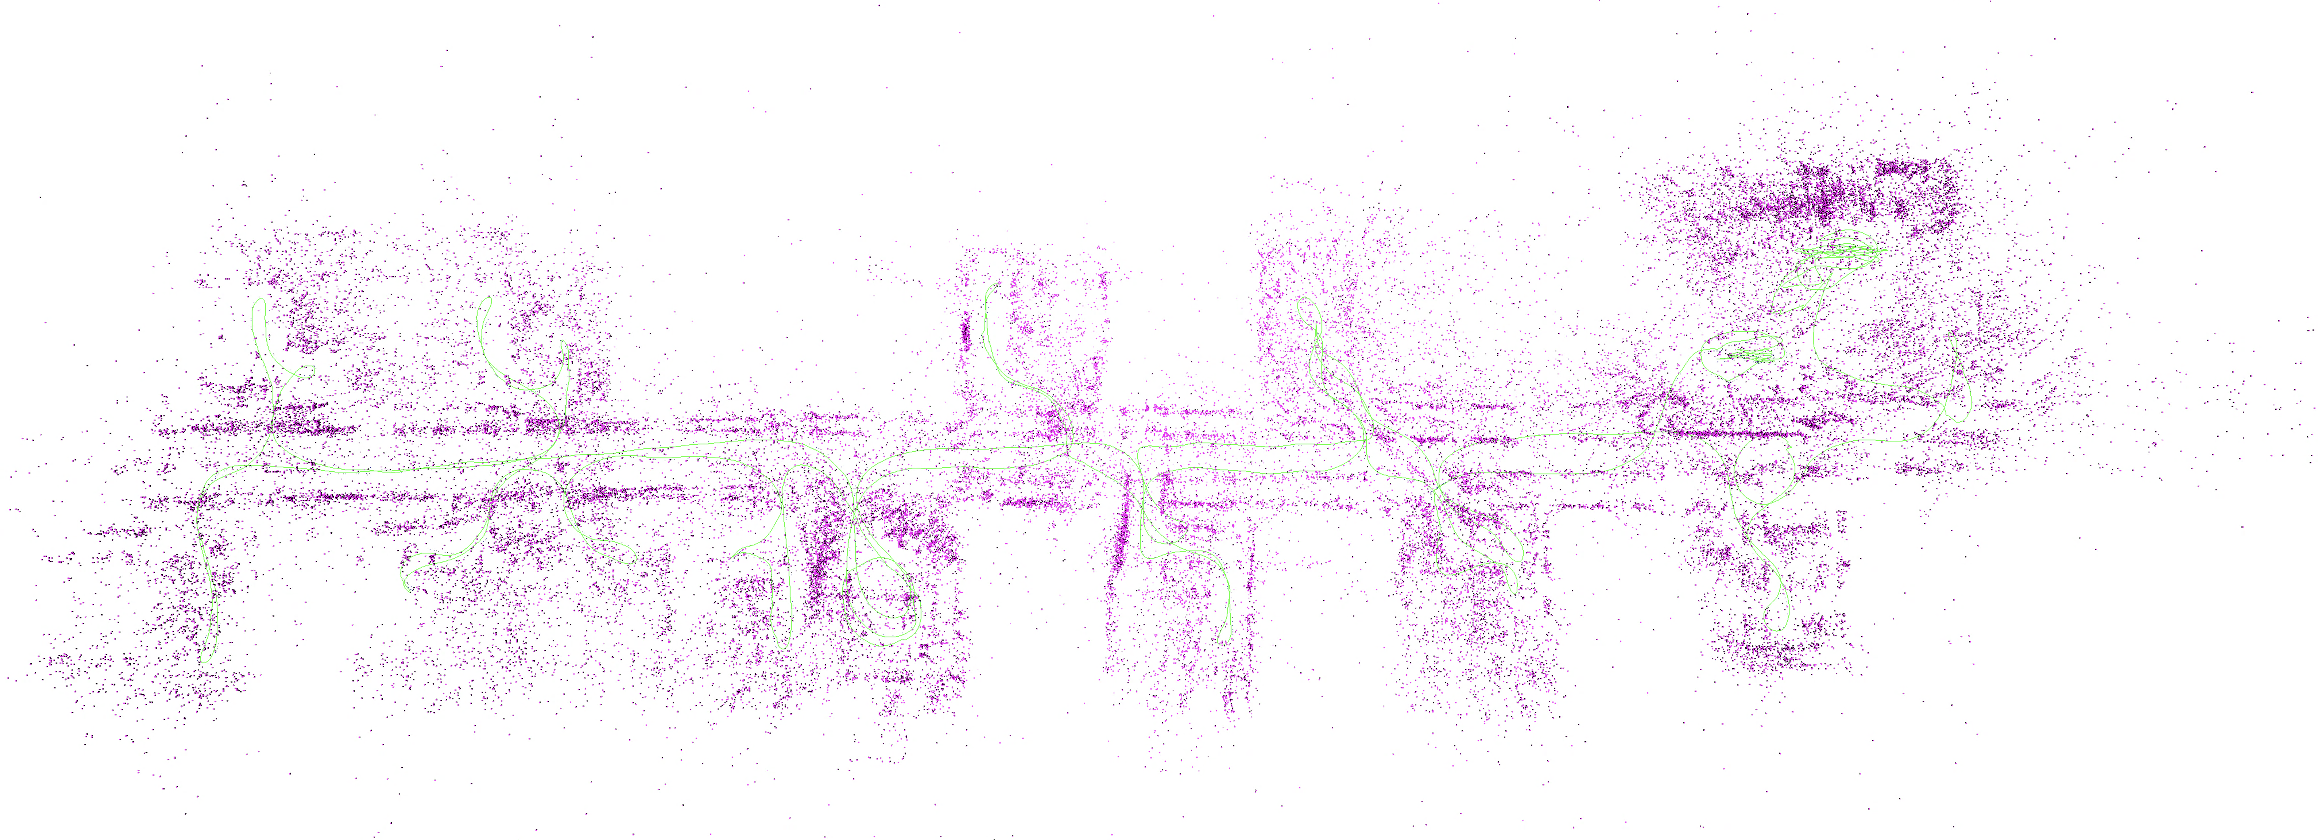
\includegraphics[width=0.9\linewidth]{Img/tumvi-corridor2}
  \bicaption{TUM-VI 数据集走廊场景下的建图与定位轨迹结果}{Mapping and localization trajectory results in the corridor scene of the TUM-VI dataset}
  \label{fig:tumvi_corridor}
\end{figure*}

\begin{table}[H]
\centering
\bicaption{EuRoC 数据集轨迹精度对比（ATE RMSE，单位：m）}{Trajectory accuracy on EuRoC dataset (ATE RMSE, unit: m)}
\label{tab:trajectory_accuracy}
\begin{tabular}{lccc}
\toprule
序列 & CPU & FPGA \\
\midrule
MH\_01\_easy & 0.049 & \textbf{0.042} \\
MH\_02\_easy & 0.077 & \textbf{0.034} \\
MH\_03\_medium & \textbf{0.086} & 0.127 \\
MH\_04\_difficult & 0.125 & \textbf{0.113} \\
MH\_05\_difficult & 0.125 & \textbf{0.098} \\
V1\_01\_easy & \textbf{0.035} & \textbf{0.035} \\
V1\_02\_medium & \textbf{0.053} & 0.065 \\
V1\_03\_difficult & 0.082 & \textbf{0.068} \\
V2\_01\_easy & \textbf{0.046} & 0.063 \\
V2\_02\_medium & \textbf{0.075} & 0.080 \\
\midrule
\textbf{Avg} & \textbf{0.075} & \textbf{0.073} \\
\bottomrule
\end{tabular}
\end{table}

为验证硬件加速不会引入额外的数值误差，本文在 EuRoC MAV 与 TUM-VI 数据集上对比了纯软件实现与软硬协同实现的轨迹精度。表~\ref{tab:trajectory_accuracy} 与表~\ref{tab:ate_tumvi} 展示了两类数据集上的 ATE RMSE 结果，图~\ref{fig:tumvi_corridor} 给出了 TUM-VI 走廊序列的轨迹示意。可以看到，硬件加速方案的精度与软件基准保持一致，误差差异处于数值噪声范围内，验证了本文硬件实现的数值正确性与鲁棒性。

\section{计算延迟与加速比}

选取 EuRoC 数据集中的 MH\_01\_easy 序列进行测试，实验数据如表~\ref{tab:performance} 所示。Schur Kernel 的硬件实现将单次优化延迟从 2.84~ms 降低至 0.76~ms，实现 \textbf{3.74$\times$} 的加速比。得益于观测处理流水线与 SOB 编码优化，系统后端优化频率可稳定运行在 \textbf{25~Hz 以上}，满足实时性需求。

\begin{table}[H]
\centering
\bicaption{CPU 与 FPGA 后端耗时对比}{Latency comparison between CPU and FPGA backend}
\label{tab:performance}
\begin{tabular}{lccc}
\toprule
模块 & CPU 耗时 (ms) & FPGA 耗时 (ms) & 加速比 \\
\midrule
Schur Kernel & 2.84 & \textbf{0.76} & \textbf{3.74$\times$} \\
\bottomrule
\end{tabular}
\end{table}

\section{资源利用率分析}

表~\ref{tab:resource_comparison} 展示了本文与同类 FPGA 加速方案的资源占用与能效对比。本文仅将后端 Schur Kernel（Hessian 构建 + Schur 消元）部署于 PL，其余系统控制与前端仍由 PS 端完成（包括滑动窗口管理、特征跟踪/匹配、状态预测与优化迭代控制等）；对比表中的外部工作均为同类后端或 BA/SLAM 加速器在 FPGA 上的实现，统计范围为 FPGA 芯片上资源占用。表中 Liu Q~\cite{liu2022energy}、Liu Q~\cite{liu2020pi}、Liu W~\cite{liu2021archytas} 与 Guo R~\cite{guo2022fpga} 均属于优化法后端方案，而 Gan Y~\cite{gan2021eudoxus} 为滤波法后端方案；本文在问题建模上采用优化法，在问题求解上采用滤波法的 EKF 更新，实现了优化建模与滤波求解的结合。优化法通常通过构建全局代价函数并求解批量最小二乘问题，而滤波法则以递推更新方式进行状态估计并强调线性化的逐步更新特性。由于软硬分工边界不同，资源规模存在差异，本文重点强调后端核心计算的协同设计与资源效率，尤其在 BRAM 占用方面显著优于同类工作，这得益于 SOB 编码对存储空间的优化。

为进一步体现能效优势，表中补充了帧率、功耗与单帧能耗（功耗/帧率）。其中帧率与功耗数据均在仅运行后端方法的条件下测得，反映该后端模块在对应平台上的极限性能。单帧能耗反映处理一帧所需能量，能够抵消不同平台帧率差异带来的偏置。可以看到，本文方案在保持较高帧率的同时，单帧能耗最低（19.1~mJ），说明本文方案在能效方面优势更为突出。

\begin{table*}[h!t]
\centering
\bicaption{与同类 FPGA 后端加速方案深度对比}{In-depth comparison with peer FPGA backend accelerators}
\label{tab:resource_comparison}
\begin{tabular}{lcccccc}
\toprule
资源类型 & Liu Q \cite{liu2022energy} & Gan Y \cite{gan2021eudoxus} & Liu Q \cite{liu2020pi} & Liu W \cite{liu2021archytas} & Guo R \cite{guo2022fpga} & \textbf{Ours} \\
\midrule
LUT  & 144108 & 350671 & 118995 & 136432 & 23489  & 114305 \\
FF   & 172935 & 239347 & 142411 & 163006 & 22696  & 155211 \\
DSP  & 869    & 1284   & 880    & 849    & 238    & 579    \\
BRAM & 1206 KB & 5787 KB & 2337 KB & 1149 KB & 230 KB & \textbf{67 KB} \\
帧率  & 60.86 FPS & 22.40 FPS & 4.00 FPS & 50 FPS & 83.3 FPS & 337 FPS \\
功耗  & 3.45 W & 8.96 W & 5.50 W & 5.00 W & N/A & 6.45 W \\
单帧能耗  & 56.7 mJ & 400 mJ & 1375 mJ & 100 mJ & N/A & \textbf{19.1 mJ} \\
\bottomrule
\end{tabular}
\end{table*}

\section{功耗与能效分析}

为全面评估本文加速器的嵌入式部署优势，本文对 CPU 软件方案与 FPGA 硬件加速方案的功耗进行了实测对比。功耗测量采用开发板自带的电流传感器，分别记录系统在空闲状态与运行后端优化算法时的实时功率，结果如表~\ref{tab:power} 所示。由于硬件实现显著缩短了计算延迟，按照式~\eqref{eq:energy} 计算，单帧能耗显著降低，能效提升明显。

\begin{table}[H]
\centering
\bicaption{功耗对比}{Power consumption comparison}
\label{tab:power}
\begin{tabular}{lccc}
\toprule
实现方案 & 静态 (W) & 动态 (W) & 峰值 (W) \\
\midrule
ARM CPU (软件) & 6.53 & 7.04 & 7.10 \\
FPGA (硬件加速) & 6.53 & \textbf{6.80} & \textbf{6.95} \\
\bottomrule
\end{tabular}
\end{table}

\section{SOB 编码优化效果分析}

为量化稀疏观测位图（SOB）编码对系统性能的提升效果，本文对不同负载场景下的计算量、存储空间和数据传输量进行了详细分析。蒙特卡洛仿真是一种基于随机采样的统计方法，通过对随机变量进行大量重复试验，以估计系统在概率意义下的期望性能与波动范围。该方法适用于含有随机观测分布或复杂组合结构的问题，可在不穷举所有情况的前提下获得稳定的统计结论。

实验采用蒙特卡洛仿真方法：在给定 $(N_p, N_s, N_{\text{obs}})$ 配置下，随机生成满足观测数量约束的观测关联集合与 SOB 位图，并对每次随机样本计算对应的 Hessian 构建迭代次数、Schur 消元乘法次数与存储/传输开销，最终取 100 次样本的均值作为统计结果。该方法能够覆盖观测分布的随机性，避免单一轨迹或特定观测拓扑带来的偏差。稀疏率 $\rho$ 按式~\eqref{eq:sparsity_ratio} 定义，其中 $N_{\text{obs}}$ 为实际观测数，$N_p$ 为路标点数量，$N_s$ 为滑动窗口内的状态数，系数 2 对应双目相机。

\begin{equation}
\rho = \frac{N_{\text{obs}}}{N_p \times N_s \times 2}
\label{eq:sparsity_ratio}
\end{equation}

\begin{figure}[h!t]
    \centering
    % SOB 编码计算量优化效果 - 折线图
% 使用方法: % SOB 编码计算量优化效果 - 折线图
% 使用方法: % SOB 编码计算量优化效果 - 折线图
% 使用方法: \input{figures/sob_computation_chart.tex}
% 字体: 中文使用宋体（继承文档设置），英文使用 Times New Roman（newtxtext）

\usetikzlibrary{arrows.meta}
\begin{tikzpicture}
\begin{axis}[
    every node/.append style={font=\rmfamily},  % 确保使用衬线字体（Times/宋体）
    width=0.85\linewidth,
    height=5.5cm,
    xlabel={稀疏率 (\%)},
    ylabel={迭代次数},
    xmin=30, xmax=80,
    ymin=0, ymax=2200,
    xtick={37.5, 50, 62.5, 73.2},
    legend pos=north west,
    legend style={font=\small},
    grid=major,
    grid style={dashed, gray!30},
    axis lines=left,
    xlabel style={font=\small},
    ylabel style={font=\small},
    tick label style={font=\small},
]

% 朴素迭代 - 蓝色实线
\addplot[
    color=blue,
    mark=square*,
    thick,
    mark size=3pt,
] coordinates {
    (37.5, 400)
    (50.0, 1200)
    (62.5, 1600)
    (73.2, 2048)
};
\addlegendentry{朴素迭代}

% 优化迭代 - 红色虚线
\addplot[
    color=red,
    mark=triangle*,
    thick,
    dashed,
    mark size=3pt,
] coordinates {
    (37.5, 152)
    (50.0, 600)
    (62.5, 974)
    (73.2, 1433)
};
\addlegendentry{SOB 优化迭代}

\end{axis}
\end{tikzpicture}

% 字体: 中文使用宋体（继承文档设置），英文使用 Times New Roman（newtxtext）

\usetikzlibrary{arrows.meta}
\begin{tikzpicture}
\begin{axis}[
    every node/.append style={font=\rmfamily},  % 确保使用衬线字体（Times/宋体）
    width=0.85\linewidth,
    height=5.5cm,
    xlabel={稀疏率 (\%)},
    ylabel={迭代次数},
    xmin=30, xmax=80,
    ymin=0, ymax=2200,
    xtick={37.5, 50, 62.5, 73.2},
    legend pos=north west,
    legend style={font=\small},
    grid=major,
    grid style={dashed, gray!30},
    axis lines=left,
    xlabel style={font=\small},
    ylabel style={font=\small},
    tick label style={font=\small},
]

% 朴素迭代 - 蓝色实线
\addplot[
    color=blue,
    mark=square*,
    thick,
    mark size=3pt,
] coordinates {
    (37.5, 400)
    (50.0, 1200)
    (62.5, 1600)
    (73.2, 2048)
};
\addlegendentry{朴素迭代}

% 优化迭代 - 红色虚线
\addplot[
    color=red,
    mark=triangle*,
    thick,
    dashed,
    mark size=3pt,
] coordinates {
    (37.5, 152)
    (50.0, 600)
    (62.5, 974)
    (73.2, 1433)
};
\addlegendentry{SOB 优化迭代}

\end{axis}
\end{tikzpicture}

% 字体: 中文使用宋体（继承文档设置），英文使用 Times New Roman（newtxtext）

\usetikzlibrary{arrows.meta}
\begin{tikzpicture}
\begin{axis}[
    every node/.append style={font=\rmfamily},  % 确保使用衬线字体（Times/宋体）
    width=0.85\linewidth,
    height=5.5cm,
    xlabel={稀疏率 (\%)},
    ylabel={迭代次数},
    xmin=30, xmax=80,
    ymin=0, ymax=2200,
    xtick={37.5, 50, 62.5, 73.2},
    legend pos=north west,
    legend style={font=\small},
    grid=major,
    grid style={dashed, gray!30},
    axis lines=left,
    xlabel style={font=\small},
    ylabel style={font=\small},
    tick label style={font=\small},
]

% 朴素迭代 - 蓝色实线
\addplot[
    color=blue,
    mark=square*,
    thick,
    mark size=3pt,
] coordinates {
    (37.5, 400)
    (50.0, 1200)
    (62.5, 1600)
    (73.2, 2048)
};
\addlegendentry{朴素迭代}

% 优化迭代 - 红色虚线
\addplot[
    color=red,
    mark=triangle*,
    thick,
    dashed,
    mark size=3pt,
] coordinates {
    (37.5, 152)
    (50.0, 600)
    (62.5, 974)
    (73.2, 1433)
};
\addlegendentry{SOB 优化迭代}

\end{axis}
\end{tikzpicture}

    \bicaption{SOB 编码计算量优化效果}{Computation reduction by SOB encoding}
    \label{fig:sob_computation}
\end{figure}

图~\ref{fig:sob_computation} 展示了 SOB 编码在不同稀疏率下的计算量优化效果。随着稀疏率增大，观测逐渐密集，优化带来的相对收益逐步降低，但在常见稀疏区间 40\%--60\% 仍保持显著优势。这一区间的观测分布既体现了稀疏性，又保留了足够数量的有效观测，使得跳零计算与有效负载之间取得更好的平衡。在典型场景（150 个路标点、600 个有效观测、稀疏率 50\%）下，Hessian 构建阶段的迭代次数从 1{,}200 次降至 600 次，节省 50\% 的计算量；舒尔消元阶段的 $\mathbf{H}_{pm} \times \mathbf{H}_{mm}^{-1}$ 矩阵乘法次数从 600 次降至 433 次，$\mathbf{H}_{pp}$ 矩阵更新次数从 2{,}400 次降至 1{,}401 次，综合节省约 40\% 的浮点运算。由于流水线中乘加与累加路径占比最高，该收益能够直接转化为后端时延的降低与吞吐提升。

SOB 编码对交叉项矩阵 $\mathbf{H}_{pm}$ 的存储空间和 DMA 传输量也有显著优化。由于每个有效的 $6 \times 3$ 子块占用 144 字节（18 个 FP64），跳过无效观测可直接减少存储和传输开销。表~\ref{tab:sob_summary} 汇总了典型场景下 SOB 编码的综合优化效果。通过协同优化计算、存储和传输三个维度，系统总浮点运算量从 1.687M 降至 924.3K，降低约 45\%，显著提升了硬件加速器的整体效率。

进一步地，从存储访问角度看，SOB 编码使得 Hessian 子块的写入由“固定稠密遍历”转为“按观测触发的稀疏写入”。在传统稠密写入策略下，硬件需对每个 $(\text{state},\text{point})$ 组合依次更新相应子块，即使该观测不存在也会触发无效写端口访问与写回，导致 BRAM 多端口冲突与写入仲裁开销增大。采用 SOB 编码后，写入行为仅在对应观测位为 1 时触发，写地址由位图解析即时生成，显著降低了并发写请求密度与端口冲突概率，从而改善了存储访问的时序收敛特性。与此同时，稀疏写入使得 DMA 输出呈“有效块连续”的流式特征，避免在总线端出现周期性峰值突发，有助于降低带宽峰值并提升传输稳定性。该特性在移动端平台尤为关键，可在相同带宽预算下维持更高的后端更新频率，并为前端传感器数据流预留充足的带宽裕量。此外，稀疏写入还降低了片上缓存的无效数据覆盖概率，使有效子块在缓存中的驻留时间更长，有利于提高缓存命中率并降低读写抖动，进一步提升流水线的稳定性与可预测性。

\begin{table}[h!t]
\centering
\bicaption{典型场景综合优化效果}{Overall optimization in typical scenario}\label{tab:sob_summary}
\begin{tabular}{lccc}
\toprule
优化维度 & 朴素方法 & SOB 优化 & 节省比例 \\
\midrule
雅可比计算浮点运算 & 901.2K & \textbf{450.5K} & \textbf{50.01\%} \\
Schur 消元浮点运算 & 785.4K & \textbf{473.8K} & \textbf{39.67\%} \\
$\mathbf{H}_{pm}$ 存储 & 84.38 KB & \textbf{60.95 KB} & \textbf{27.77\%} \\
DMA 输出传输 & 103.12 KB & \textbf{79.70 KB} & \textbf{22.72\%} \\
\midrule
\textbf{总浮点运算} & \textbf{1.687M} & \textbf{924.3K} & \textbf{45.18\%} \\
\bottomrule
\end{tabular}
\end{table}

\section{真实场景测试}

为验证本文加速方案在实际机器人系统中的作业能力，我们将系统部署于集成的移动机器人异构计算平台。如图~\ref{fig:VIOboard} 所示，该板卡搭载双目摄像头与 IMU 传感器，核心处理单元为 XCZU19EG，提供充足的 PS 与 PL 资源支持 Schur Kernel 加速架构。系统端到端流程包括：传感器同步采集、前端特征跟踪与匹配、滑动窗口状态管理、后端 Schur Kernel 计算以及结果回写与状态更新。为保证实验可复现性，测试过程中固定相机内参与外参标定参数，并对传感器时间戳进行对齐处理，确保视觉与惯性数据在同一时间基准下进入后端优化模块。

\begin{figure}[h!t]
\centering
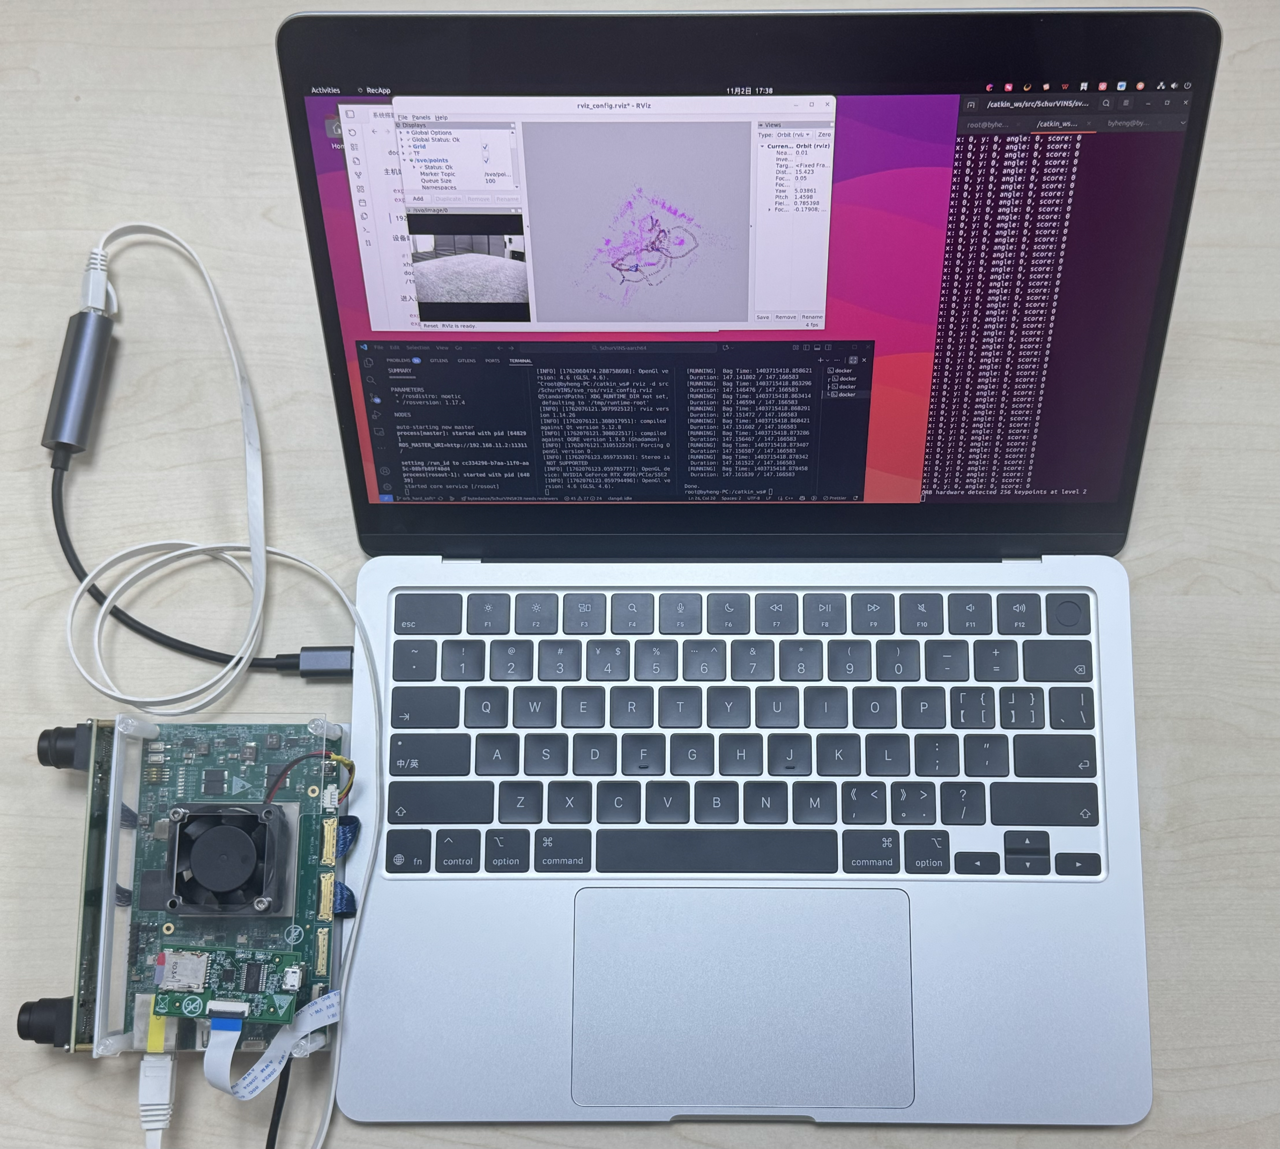
\includegraphics[width=0.8\linewidth]{Img/VIOboard}
\bicaption{搭载双目摄像头与 IMU 的嵌入式开发板}{Embedded development board equipped with stereo cameras and IMU}
\label{fig:VIOboard}
\end{figure}

测试环境选择在户外真实场景进行，以验证系统在复杂动态环境下的定位与建图鲁棒性。如图~\ref{fig:outdoortest} 所示，实验场景包含光照变化、纹理稠密与纹理稀疏区域交替出现等典型因素。系统在全程运行中保持连续建图与位姿输出，轨迹整体平滑且与环境结构一致，表明软硬协同后端能够在实际场景下维持稳定的优化效果。

\begin{figure}[h!t]
\centering
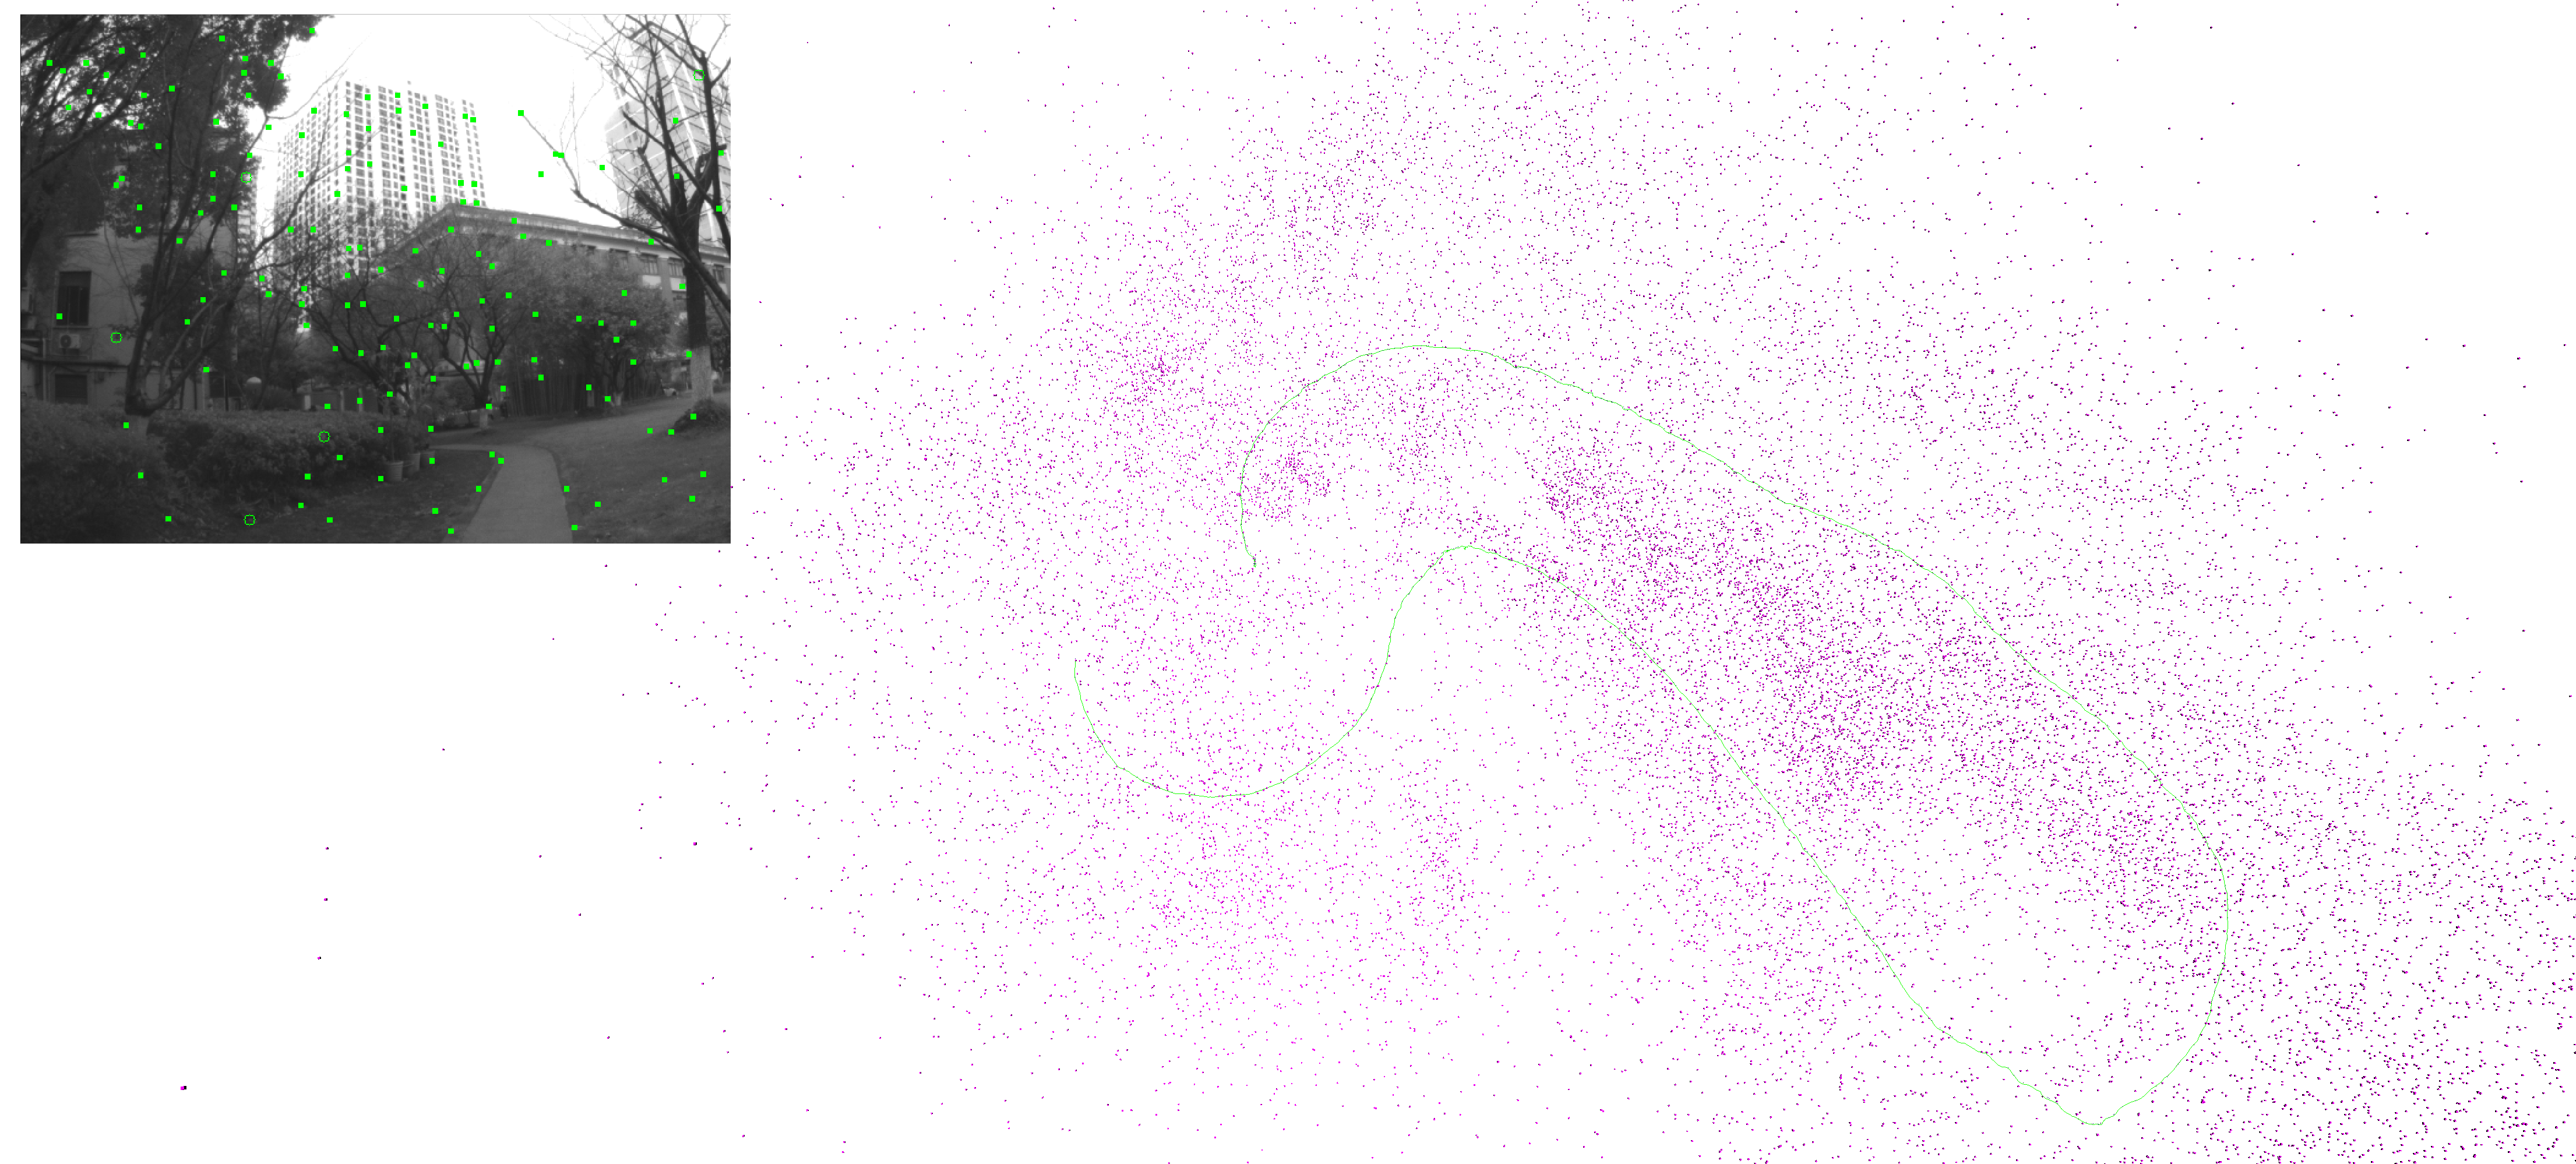
\includegraphics[width=0.9\linewidth]{Img/outdoor}
\bicaption{户外真实场景下的定位与建图测试结果}{Localization and mapping results in an outdoor real-world scene}
\label{fig:outdoortest}
\end{figure}

% \begin{figure}[h!t]
% \centering
% 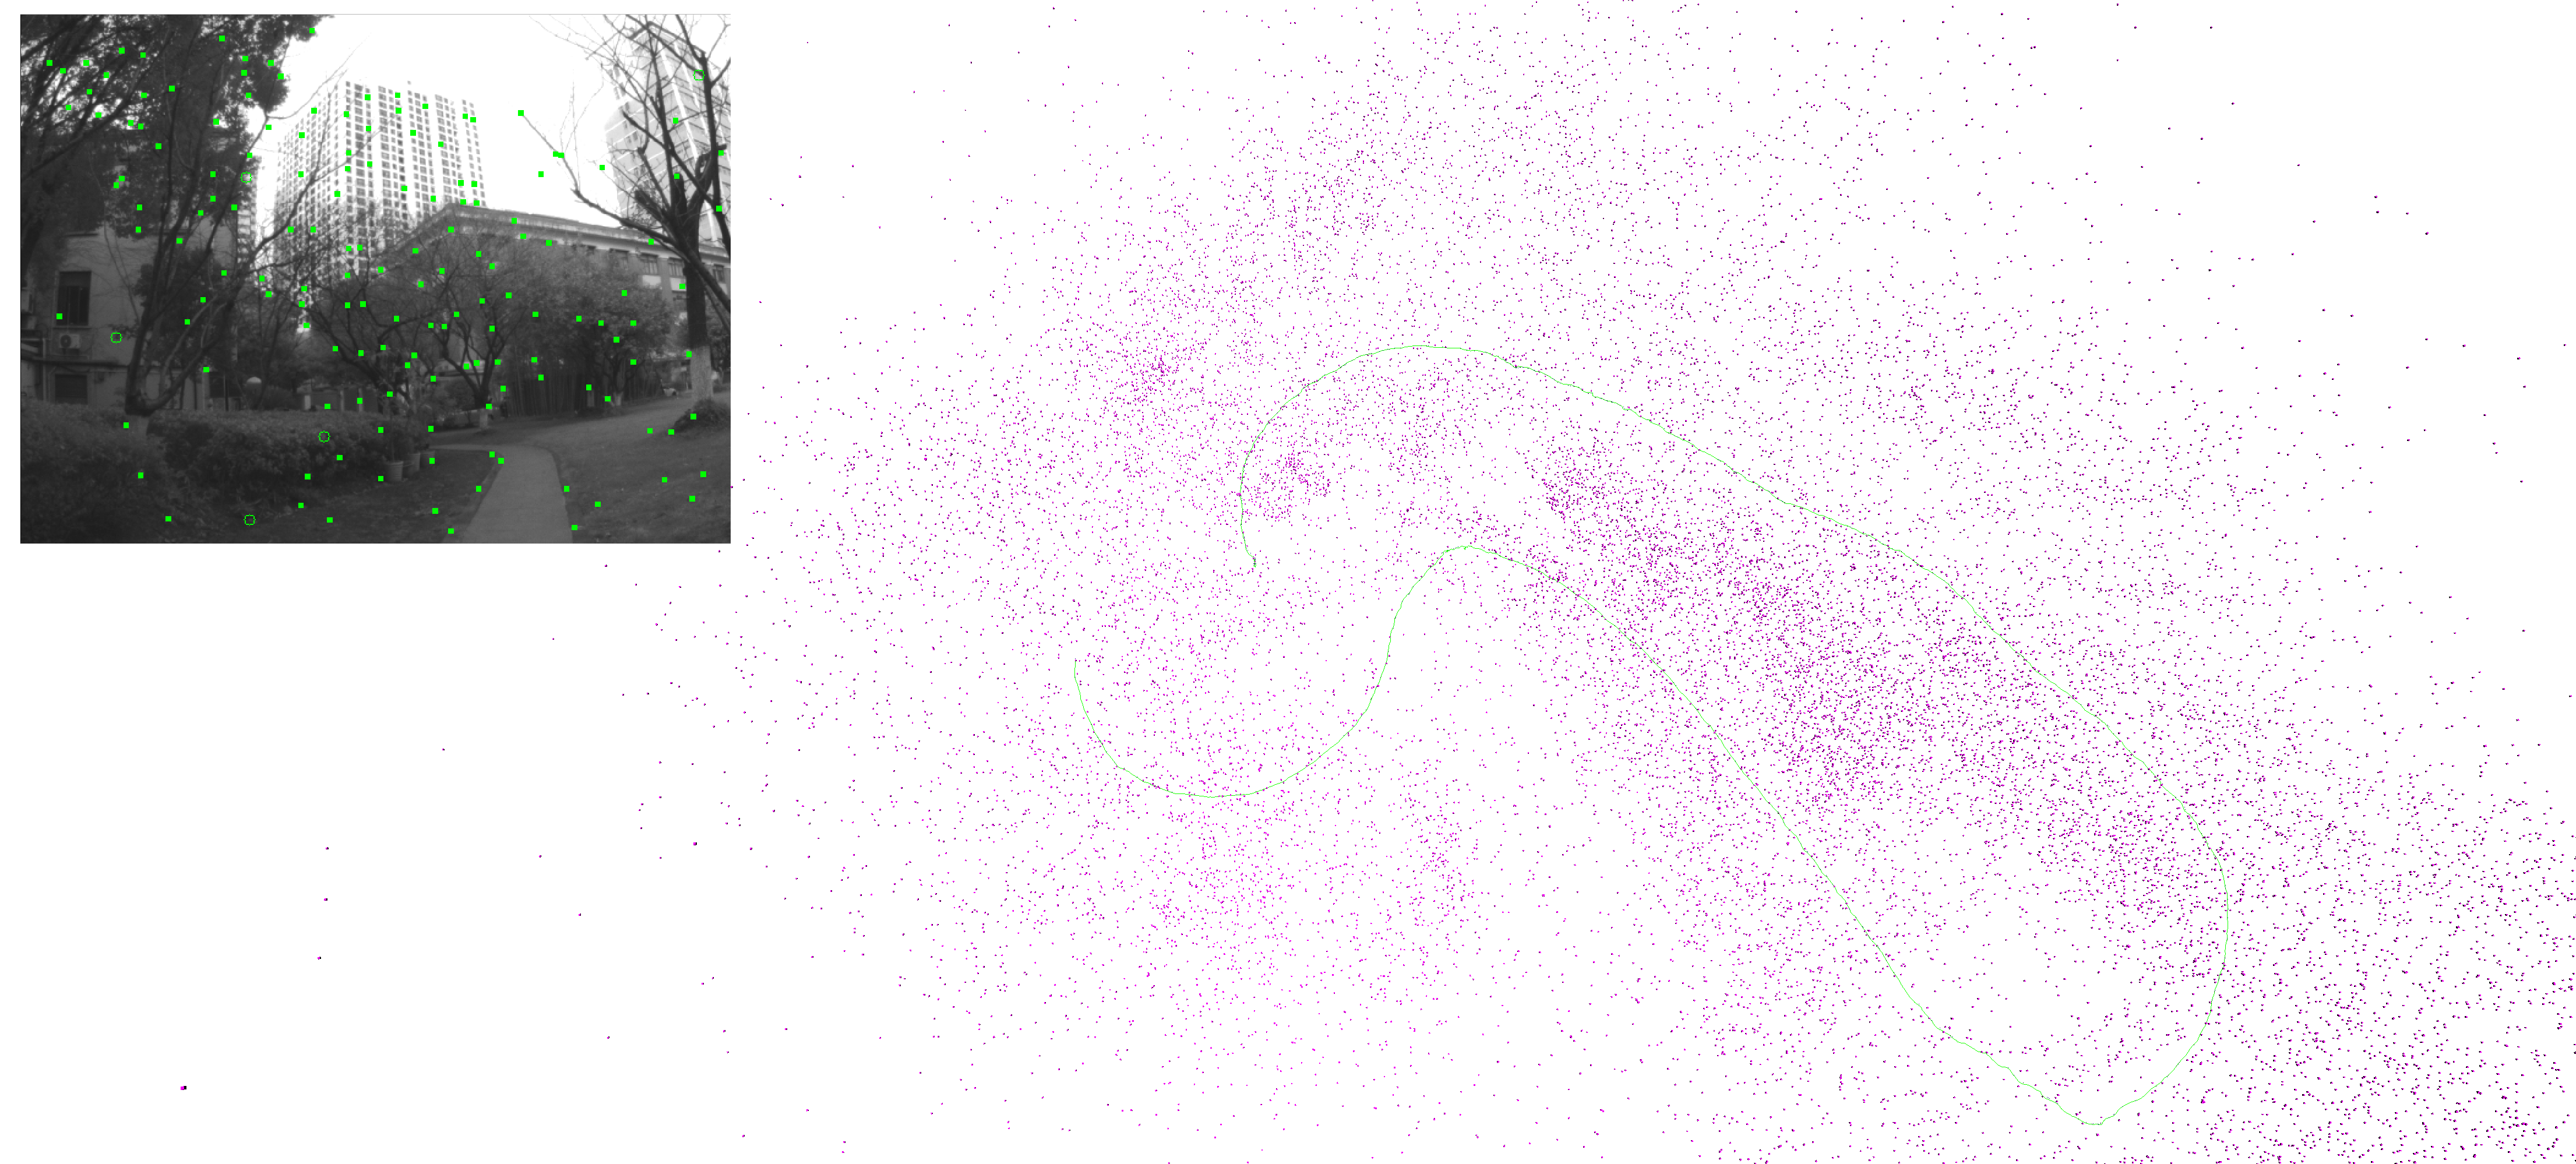
\includegraphics[width=0.9\linewidth]{Img/outdoor}
% \bicaption{户外}{outdoor real-world scene}
% \label{fig:outdoor}
% \end{figure}

在处理 20~Hz 采集频率的双目观测流时，本文软硬协同加速架构展现了良好的作业潜力。实验结果显示，系统后端优化模块的计算频率可稳定在 \textbf{25~Hz 以上}，即便在长距离移动过程中也能保持稳定的实时响应。与此同时，后端计算的延迟波动较小，说明所提出的流水化与稀疏门控机制能够有效抑制由观测稀疏性变化带来的性能抖动。综合而言，真实场景实验验证了本文加速器在工程部署中的可行性与实时性，为后续面向移动机器人与嵌入式平台的应用奠定了基础。

\section{本章小结}

本章完成了基于 XCZU19EG 平台的实验验证，结果表明所设计的 Schur Kernel 加速器在 EuRoC MAV 与 TUM-VI 数据集上保持了与软件基准一致的定位精度，同时实现了 \textbf{3.74$\times$} 的后端加速比。SOB 编码在计算、存储与传输三个维度带来显著优化，使 BRAM 占用降至 67~KB，并在功耗与能效方面体现出嵌入式部署优势，验证了本文方案在真实场景下的可用性与实时性。